\chapter{数论}

\index{number theory}

\key{数论}是研究整数的数学分支。数论是一门引人入胜的学科，因为许多与整数有关的问题乍看十分简单，解决起来却非常困难。

例如，考虑方程：
\[x^3 + y^3 + z^3 = 33\]
很容易找到满足该方程的三个实数 $x$、$y$、$z$。例如，可以取
\[
\begin{array}{lcl}
x = 3, \\
y = \sqrt[3]{3}, \\
z = \sqrt[3]{3}.\\
\end{array}
\]
然而，在本书原稿写作时，是否存在满足该方程的三个\emph{整数} $x$、$y$、$z$ 仍是数论中的一个公开问题 \cite{bec07}。

本章重点介绍数论中的基本概念与算法。除非另有说明，本章中的所有数都假定为整数。

\section{素数与因数}

\index{divisibility}
\index{factor}
\index{divisor}

如果 $a$ 整除 $b$，就称 $a$ 是 $b$ 的\key{因数}或\key{约数}。若 $a$ 是 $b$ 的因数，记作 $a \mid b$；否则记作 $a \nmid b$。例如，24 的因数为 1、2、3、4、6、8、12、24。

\index{prime}
\index{prime decomposition}

若 $n>1$ 的正因数只有 1 和 $n$，则称 $n$ 为\key{素数}。例如，7、19、41 是素数，而 35 不是素数，因为 $5 \cdot 7 = 35$。每个 $n>1$ 都有唯一的\key{质因数分解}
\[ n = p_1^{\alpha_1} p_2^{\alpha_2} \cdots p_k^{\alpha_k},\]
其中 $p_1,p_2,\ldots,p_k$ 是互不相同的素数，$\alpha_1,\alpha_2,\ldots,\alpha_k$ 是正整数。例如，84 的质因数分解为
\[84 = 2^2 \cdot 3^1 \cdot 7^1.\]

数 $n$ 的\key{因数个数}为
\[\tau(n)=\prod_{i=1}^k (\alpha_i+1),\]
因为对于每个素数 $p_i$，它在一个因数中出现的次数有 $\alpha_i+1$ 种选择。例如，84 的因数个数为 $\tau(84)=3 \cdot 2 \cdot 2 = 12$。这些因数是 1、2、3、4、6、7、12、14、21、28、42、84。

数 $n$ 的\key{因数和}为
\[\sigma(n)=\prod_{i=1}^k (1+p_i+\ldots+p_i^{\alpha_i}) = \prod_{i=1}^k \frac{p_i^{a_i+1}-1}{p_i-1},\]
后一个等式来自等比数列求和公式。例如，84 的因数和为
\[\sigma(84)=\frac{2^3-1}{2-1} \cdot \frac{3^2-1}{3-1} \cdot \frac{7^2-1}{7-1} = 7 \cdot 4 \cdot 8 = 224.\]

数 $n$ 的\key{因数乘积}为
\[\mu(n)=n^{\tau(n)/2},\]
因为可以把所有因数配成 $\tau(n)/2$ 对，每对的乘积均为 $n$。例如，84 的因数可配成 $1 \cdot 84$、$2 \cdot 42$、$3 \cdot 28$ 等，因此因数乘积为 $\mu(84)=84^6=351298031616$。

\index{perfect number}

若 $n=\sigma(n)-n$，即 $n$ 等于它在 1 到 $n-1$ 之间所有因数之和，则称 $n$ 为\key{完全数}。例如，28 是完全数，因为 $28=1+2+4+7+14$。

\subsubsection{素数的数量}

很容易证明素数有无穷多个。如果素数只有有限多个，就可以构造包含全部素数的集合 $P=\{p_1,p_2,\ldots,p_n\}$，例如 $p_1=2$、$p_2=3$、$p_3=5$，依此类推。然而，利用 $P$ 可以构造一个新的素数
\[p_1 p_2 \cdots p_n+1\]
它大于 $P$ 中的所有元素。这产生了矛盾，因此素数必有无穷多个。

\subsubsection{素数密度}

素数密度描述素数在整数中出现的频繁程度。令 $\pi(n)$ 表示 1 到 $n$ 之间的素数个数。例如，$\pi(10)=4$，因为 1 到 10 之间有 2、3、5、7 共 4 个素数。

可以证明
\[\pi(n) \approx \frac{n}{\ln n},\]
这表明素数相当常见。例如，1 到 $10^6$ 之间的素数个数为 $\pi(10^6)=78498$，而 $10^6 / \ln 10^6 \approx 72382$。

\subsubsection{猜想}

关于素数有许多\emph{猜想}。人们普遍认为这些猜想成立，但至今尚无人能够证明。著名的例子包括：

\begin{itemize}
\index{Goldbach's conjecture}
\item \key{哥德巴赫猜想}：每个偶数 $n>2$ 都能表示为 $n=a+b$，其中 $a$ 和 $b$ 均为素数。
\index{twin prime}
\item \key{孪生素数猜想}：形如 $\{p,p+2\}$ 且 $p$ 与 $p+2$ 均为素数的数对有无穷多组。
\index{Legendre's conjecture}
\item \key{Legendre 猜想}：对于任意正整数 $n$，$n^2$ 与 $(n+1)^2$ 之间总存在一个素数。
\end{itemize}

\subsubsection{基础算法}

如果 $n$ 不是素数，就可以写成 $a \cdot b$，其中 $a \le \sqrt n$ 或 $b \le \sqrt n$，因此它在 $2$ 到 $\lfloor \sqrt n \rfloor$ 之间一定有一个因数。利用这一观察，可以在 $O(\sqrt n)$ 时间内判断一个数是否为素数，也可以求出它的质因数分解。

下面的函数 \texttt{prime} 判断给定的 $n$ 是否为素数。函数尝试用 $2$ 到 $\lfloor \sqrt n \rfloor$ 之间的所有数去除 $n$；如果没有一个能够整除 $n$，则 $n$ 为素数。

\begin{lstlisting}
bool prime(int n) {
    if (n < 2) return false;
    for (int x = 2; x*x <= n; x++) {
        if (n%x == 0) return false;
    }
    return true;
}
\end{lstlisting}

\noindent
下面的函数 \texttt{factors} 构造一个保存 $n$ 的质因数分解的向量。函数不断用 $n$ 的质因数除它，并把这些质因数加入向量。当剩余的 $n$ 在 $2$ 到 $\lfloor \sqrt n \rfloor$ 之间不再有因数时，过程结束。若此时 $n>1$，它就是最后一个素因数。

\begin{lstlisting}
vector<int> factors(int n) {
    vector<int> f;
    for (int x = 2; x*x <= n; x++) {
        while (n%x == 0) {
            f.push_back(x);
            n /= x;
        }
    }
    if (n > 1) f.push_back(n);
    return f;
}
\end{lstlisting}

注意，每个素因数在向量中出现的次数等于它在原数的质因数分解中的指数。例如，$24=2^3 \cdot 3$，因此函数返回 $[2,2,2,3]$。

\subsubsection{Eratosthenes 筛法}

\index{sieve of Eratosthenes}

\key{Eratosthenes 筛法}
%\footnote{Eratosthenes (c. 276 BC -- c. 194 BC) was a Greek mathematician.}
是一种预处理算法。它构造一个数组，使我们能够高效判断 $2 \ldots n$ 之间的给定整数是否为素数；如果不是，还能找到它的一个素因数。

算法构造数组 $\texttt{sieve}$，使用其中位置 $2,3,\ldots,n$。$\texttt{sieve}[k]=0$ 表示 $k$ 是素数；$\texttt{sieve}[k] \neq 0$ 表示 $k$ 不是素数，并且 $\texttt{sieve}[k]$ 是它的一个素因数。

算法依次遍历 $2 \ldots n$。每当发现一个新素数 $x$，就把 $x$ 的所有倍数（$2x,3x,4x,\ldots$）标记为合数，因为它们都能被 $x$ 整除。

例如，当 $n=20$ 时，数组如下：

\begin{center}
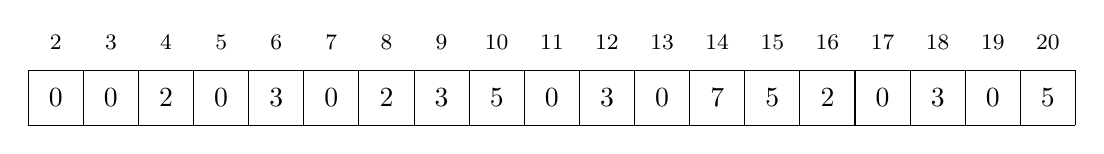
\begin{tikzpicture}[scale=0.7]
\draw (0,0) grid (19,1);

\node at (0.5,0.5) {$0$};
\node at (1.5,0.5) {$0$};
\node at (2.5,0.5) {$2$};
\node at (3.5,0.5) {$0$};
\node at (4.5,0.5) {$3$};
\node at (5.5,0.5) {$0$};
\node at (6.5,0.5) {$2$};
\node at (7.5,0.5) {$3$};
\node at (8.5,0.5) {$5$};
\node at (9.5,0.5) {$0$};
\node at (10.5,0.5) {$3$};
\node at (11.5,0.5) {$0$};
\node at (12.5,0.5) {$7$};
\node at (13.5,0.5) {$5$};
\node at (14.5,0.5) {$2$};
\node at (15.5,0.5) {$0$};
\node at (16.5,0.5) {$3$};
\node at (17.5,0.5) {$0$};
\node at (18.5,0.5) {$5$};

\footnotesize

\node at (0.5,1.5) {$2$};
\node at (1.5,1.5) {$3$};
\node at (2.5,1.5) {$4$};
\node at (3.5,1.5) {$5$};
\node at (4.5,1.5) {$6$};
\node at (5.5,1.5) {$7$};
\node at (6.5,1.5) {$8$};
\node at (7.5,1.5) {$9$};
\node at (8.5,1.5) {$10$};
\node at (9.5,1.5) {$11$};
\node at (10.5,1.5) {$12$};
\node at (11.5,1.5) {$13$};
\node at (12.5,1.5) {$14$};
\node at (13.5,1.5) {$15$};
\node at (14.5,1.5) {$16$};
\node at (15.5,1.5) {$17$};
\node at (16.5,1.5) {$18$};
\node at (17.5,1.5) {$19$};
\node at (18.5,1.5) {$20$};

\end{tikzpicture}
\end{center}

以下代码实现 Eratosthenes 筛法，并假定 \texttt{sieve} 的所有元素初始均为零。

\begin{lstlisting}
for (int x = 2; x <= n; x++) {
    if (sieve[x]) continue;
    for (int u = 2*x; u <= n; u += x) {
        sieve[u] = x;
    }
}
\end{lstlisting}

对于每个 $x$，算法的内层循环执行 $n/x$ 次。因此，算法运行时间的一个上界是调和和
\[\sum_{x=2}^n n/x = n/2 + n/3 + n/4 + \cdots + n/n = O(n \log n).\]

\index{harmonic sum}

实际上，算法更为高效，因为只有当 $x$ 为素数时才会执行内层循环。可以证明，算法的运行时间仅为 $O(n \log \log n)$，非常接近 $O(n)$。

\subsubsection{Euclid 算法}

\index{greatest common divisor}
\index{least common multiple}
\index{Euclid's algorithm}

数 $a$ 与 $b$ 的\key{最大公约数} $\gcd(a,b)$，是同时整除 $a$ 和 $b$ 的最大整数；$a$ 与 $b$ 的\key{最小公倍数} $\textrm{lcm}(a,b)$，是同时被 $a$ 和 $b$ 整除的最小正整数。例如，$\gcd(24,36)=12$，$\textrm{lcm}(24,36)=72$。

最大公约数与最小公倍数满足：
\[\textrm{lcm}(a,b)=\frac{ab}{\textrm{gcd}(a,b)}\]

\key{Euclid 算法}\footnote{Euclid 是约生活于公元前 300 年的希腊数学家。这可能是历史上最早的已知算法。}可以高效求出两个数的最大公约数。算法基于公式：
\begin{equation*}
    \textrm{gcd}(a,b) = \begin{cases}
               a        & b = 0\\
               \textrm{gcd}(b,a \bmod b) & b \neq 0\\
           \end{cases}
\end{equation*}

例如，
\[\textrm{gcd}(24,36) = \textrm{gcd}(36,24)
= \textrm{gcd}(24,12) = \textrm{gcd}(12,0)=12.\]

算法可以实现如下：
\begin{lstlisting}
int gcd(int a, int b) {
    if (b == 0) return a;
    return gcd(b, a%b);
}
\end{lstlisting}

可以证明，Euclid 算法的时间复杂度为 $O(\log n)$，其中 $n=\min(a,b)$。当 $a$、$b$ 是相邻 Fibonacci 数时达到最坏情况。例如，
\[\textrm{gcd}(13,8)=\textrm{gcd}(8,5)
=\textrm{gcd}(5,3)=\textrm{gcd}(3,2)=\textrm{gcd}(2,1)=\textrm{gcd}(1,0)=1.\]

\subsubsection{Euler 函数}

\index{coprime}
\index{Euler's totient function}

若 $\textrm{gcd}(a,b)=1$，则称 $a$ 与 $b$ \key{互质}。\key{Euler 函数} $\varphi(n)$
%\footnote{Euler presented this function in 1763.}
表示 1 到 $n$ 之间与 $n$ 互质的整数个数。例如，$\varphi(12)=4$，因为 1、5、7、11 与 12 互质。

可以根据 $n$ 的质因数分解用以下公式计算 $\varphi(n)$：
\[ \varphi(n) = \prod_{i=1}^k p_i^{\alpha_i-1}(p_i-1). \]
例如，$\varphi(12)=2^1 \cdot (2-1) \cdot 3^0 \cdot (3-1)=4$。注意，如果 $n$ 是素数，则 $\varphi(n)=n-1$。

\section{模运算}

\index{modular arithmetic}

在\key{模运算}中，数的范围被限制为 $0,1,2,\ldots,m-1$，其中 $m$ 是常数。每个数 $x$ 用 $x \bmod m$ 表示，即 $x$ 除以 $m$ 的余数。例如，当 $m=17$ 时，75 表示为 $75 \bmod 17 = 7$。

通常可以先取模再进行计算。特别地，下列公式成立：
\[
\begin{array}{rcl}
(x+y) \bmod m & = & (x \bmod m + y \bmod m) \bmod m \\
(x-y) \bmod m & = & (x \bmod m - y \bmod m) \bmod m \\
(x \cdot y) \bmod m & = & (x \bmod m \cdot y \bmod m) \bmod m \\
x^n \bmod m & = & (x \bmod m)^n \bmod m \\
\end{array}
\]

\subsubsection{快速幂取模}

经常需要高效计算 $x^n \bmod m$。利用下面的递归，可以在 $O(\log n)$ 时间内完成：
\begin{equation*}
    x^n = \begin{cases}
               1        & n = 0\\
               x^{n/2} \cdot x^{n/2} & \text{$n$ is even}\\
               x^{n-1} \cdot x & \text{$n$ is odd}
           \end{cases}
\end{equation*}

关键在于，当 $n$ 为偶数时，$x^{n/2}$ 只计算一次。因为每当 $n$ 为偶数时都会减半，这就保证了算法的时间复杂度为 $O(\log n)$。

下面的函数计算 $x^n \bmod m$：

\begin{lstlisting}
int modpow(int x, int n, int m) {
    if (n == 0) return 1%m;
    long long u = modpow(x,n/2,m);
    u = (u*u)%m;
    if (n%2 == 1) u = (u*x)%m;
    return u;
}
\end{lstlisting}

\subsubsection{Fermat 定理与 Euler 定理}

\index{Fermat's theorem}
\index{Euler's theorem}

\key{Fermat 小定理}
%\footnote{Fermat discovered this theorem in 1640.}
指出，当 $m$ 为素数且 $x$ 与 $m$ 互质时，
\[x^{m-1} \bmod m = 1\]
由此还可得到
\[x^k \bmod m = x^{k \bmod (m-1)} \bmod m.\]
更一般地，\key{Euler 定理}
%\footnote{Euler published this theorem in 1763.}
指出，当 $x$ 与 $m$ 互质时，
\[x^{\varphi(m)} \bmod m = 1\]
Fermat 小定理是 Euler 定理的推论，因为当 $m$ 为素数时，$\varphi(m)=m-1$。

\subsubsection{模逆元}

\index{modular inverse}

模 $m$ 意义下 $x$ 的逆元是满足下式的数 $x^{-1}$：
\[ x x^{-1} \bmod m = 1. \]
例如，当 $x=6$、$m=17$ 时，$x^{-1}=3$，因为 $6\cdot3 \bmod 17=1$。

利用模逆元，可以在模 $m$ 意义下进行除法，因为除以 $x$ 等价于乘以 $x^{-1}$。例如，要计算 $36/6 \bmod 17$，可以计算 $2 \cdot 3 \bmod 17$，因为 $36 \bmod 17 = 2$ 且 $6^{-1} \bmod 17 = 3$。

不过，模逆元并不总是存在。例如，当 $x=2$、$m=4$ 时，方程
\[ x x^{-1} \bmod m = 1 \]
无解，因为 2 的倍数都是偶数，模 4 的余数不可能为 1。事实上，$x^{-1} \bmod m$ 存在当且仅当 $x$ 与 $m$ 互质。

如果模逆元存在，可以用公式
\[
x^{-1} = x^{\varphi(m)-1}.
\]
当 $m$ 为素数时，公式变为
\[
x^{-1} = x^{m-2}.
\]
例如，
\[6^{-1} \bmod 17 =6^{17-2} \bmod 17 = 3.\]

利用快速幂取模算法，可以通过该公式高效计算模逆元。这个公式可由 Euler 定理推出。首先，模逆元应满足：
\[
x x^{-1} \bmod m = 1.
\]
另一方面，根据 Euler 定理，
\[
x^{\varphi(m)} \bmod m =  xx^{\varphi(m)-1} \bmod m = 1,
\]
因此 $x^{-1}$ 与 $x^{\varphi(m)-1}$ 在模 $m$ 意义下相等。

\subsubsection{计算机算术}

在程序中，无符号整数按模 $2^k$ 表示，其中 $k$ 是数据类型的位数。常见的结果是：当数值过大时会发生回绕。

例如，在 C++ 中，\texttt{unsigned int} 类型按模 $2^{32}$ 表示。下面的代码声明一个值为 $123456789$ 的 \texttt{unsigned int} 变量，再将其与自身相乘，结果为 $123456789^2 \bmod 2^{32} = 2537071545$。

\begin{lstlisting}
unsigned int x = 123456789;
cout << x*x << "\n"; // 2537071545
\end{lstlisting}

\section{求解方程}

\subsubsection*{不定方程}

\index{Diophantine equation}

\key{不定方程}
%\footnote{Diophantus of Alexandria was a Greek mathematician who lived in the 3th century.}
是形如
\[ ax + by = c, \]
的方程，其中 $a$、$b$、$c$ 为常数，需要求出 $x$、$y$，且方程中的所有数都必须是整数。例如，方程 $5x+2y=11$ 的一组解是 $x=3$、$y=-2$。

\index{extended Euclid's algorithm}

利用 Euclid 算法可以高效求解不定方程。可以扩展 Euclid 算法，使其求出满足下式的 $x$、$y$：
\[
ax + by = \textrm{gcd}(a,b)
\]

当且仅当 $c$ 能被 $\textrm{gcd}(a,b)$ 整除时，不定方程有整数解。

例如，求满足下式的 $x$、$y$：
\[
39x + 15y = 12
\]
因为 $\textrm{gcd}(39,15)=3$ 且 $3 \mid 12$，所以方程有解。Euclid 算法计算 39 与 15 的最大公约数时，产生如下调用序列：
\[
\textrm{gcd}(39,15) = \textrm{gcd}(15,9)
= \textrm{gcd}(9,6) = \textrm{gcd}(6,3)
= \textrm{gcd}(3,0) = 3 \]
它对应以下等式：
\[
\begin{array}{lcl}
39 - 2 \cdot 15 & = & 9 \\
15 - 1 \cdot 9 & = & 6 \\
9 - 1 \cdot 6 & = & 3 \\
\end{array}
\]
利用这些等式可以推出
\[
39 \cdot 2 + 15 \cdot (-5) = 3
\]
将其乘以 4，得到
\[
39 \cdot 8 + 15 \cdot (-20) = 12,
\]
所以方程的一组解为 $x=8$、$y=-20$。

不定方程的解并不唯一；已知一组解后，可以构造无穷多组解。如果 $(x,y)$ 是一组解，那么所有形如
\[(x+\frac{kb}{\textrm{gcd}(a,b)},y-\frac{ka}{\textrm{gcd}(a,b)})\]
的数对也都是解，其中 $k$ 为任意整数。

\subsubsection{中国剩余定理}

\index{Chinese remainder theorem}

\key{中国剩余定理}用于求解形如
\[
\begin{array}{lcl}
x & = & a_1 \bmod m_1 \\
x & = & a_2 \bmod m_2 \\
\cdots \\
x & = & a_n \bmod m_n \\
\end{array}
\]
的方程组，其中 $m_1,m_2,\ldots,m_n$ 两两互质。

令 $x^{-1}_m$ 表示 $x$ 模 $m$ 的逆元，并令
\[ X_k = \frac{m_1 m_2 \cdots m_n}{m_k}.\]
使用这一记号，方程组的一组解为
\[x = a_1 X_1 {X_1}^{-1}_{m_1} + a_2 X_2 {X_2}^{-1}_{m_2} + \cdots + a_n X_n {X_n}^{-1}_{m_n}.\]
在该解中，对于每个 $k=1,2,\ldots,n$，都有
\[a_k X_k {X_k}^{-1}_{m_k} \bmod m_k = a_k,\]
因为
\[X_k {X_k}^{-1}_{m_k} \bmod m_k = 1.\]
而和式中的其他各项都能被 $m_k$ 整除，不影响余数，因此 $x \bmod m_k = a_k$。

例如，方程组
\[
\begin{array}{lcl}
x & = & 3 \bmod 5 \\
x & = & 4 \bmod 7 \\
x & = & 2 \bmod 3 \\
\end{array}
\]
的一组解为
\[ 3 \cdot 21 \cdot 1 + 4 \cdot 15 \cdot 1 + 2 \cdot 35 \cdot 2 = 263.\]

找到一组解 $x$ 后，可以构造无穷多组其他解，因为所有形如
\[x+m_1 m_2 \cdots m_n\]
的数都是解。

\section{其他结论}

\subsubsection{Lagrange 四平方定理}

\index{Lagrange's theorem}

\key{Lagrange 四平方定理}
%\footnote{J.-L. Lagrange (1736--1813) was an Italian mathematician.}
指出，每个正整数都能表示为四个平方数之和，即 $a^2+b^2+c^2+d^2$。例如，123 可以表示为 $8^2+5^2+5^2+3^2$。

\subsubsection{Zeckendorf 定理}

\index{Zeckendorf's theorem}
\index{Fibonacci number}

\key{Zeckendorf 定理}
%\footnote{E. Zeckendorf published the theorem in 1972 \cite{zec72}; however, this was not a new result.}
指出，每个正整数都有唯一一种表示，可以写成若干个互不相同且任意两个都不相邻的 Fibonacci 数之和。例如，74 可以表示为 $55+13+5+1$。

\subsubsection{勾股数}

\index{Pythagorean triple}
\index{Euclid's formula}

\key{勾股数}是满足勾股定理 $a^2+b^2=c^2$ 的三元组 $(a,b,c)$，即存在一条三边长分别为 $a$、$b$、$c$ 的直角三角形。例如，$(3,4,5)$ 是一组勾股数。

若 $(a,b,c)$ 是一组勾股数，则当 $k>1$ 时，所有 $(ka,kb,kc)$ 也都是勾股数。若 $a$、$b$、$c$ 的最大公约数为 1，则称这组勾股数为\emph{本原勾股数}。所有勾股数都可由本原勾股数乘以某个倍数 $k$ 得到。

\key{Euclid 公式}可以生成所有本原勾股数。每组本原勾股数都形如
\[(n^2-m^2,2nm,n^2+m^2),\]
其中 $0<m<n$，$n$ 与 $m$ 互质，并且二者至少有一个是偶数。例如，当 $m=1$、$n=2$ 时，该公式产生最小的勾股数
\[(2^2-1^2,2\cdot2\cdot1,2^2+1^2)=(3,4,5).\]

\subsubsection{Wilson 定理}

\index{Wilson's theorem}

\key{Wilson 定理}
%\footnote{J. Wilson (1741--1793) was an English mathematician.}
指出，$n$ 为素数当且仅当
\[(n-1)! \bmod n = n-1.\]
例如，11 是素数，因为
\[10! \bmod 11 = 10,\]
而 12 不是素数，因为
\[11! \bmod 12 = 0 \neq 11.\]

因此，Wilson 定理可用于判断一个数是否为素数。不过在实践中，该定理无法用于很大的 $n$，因为当 $n$ 很大时，计算 $(n-1)!$ 十分困难。
